% !TeX root = ../article-enso.tex

\section{Numerical models}
\label{sec:model-des}

Mechanistic ecosystem models such as APECOSM used here are valuable tools to understand the mechanisms that govern the variability of ocean ecosystems. They generally require physical and biogeochemical forcings (temperature, currents, oxygen, low-trophic levels concentration) as inputs. In the present study, the APECOSM model is forced by the data from a coupled physical and biogeochemical simulation, which is described in section \ref{sec:nemo}. The ecosystem simulation is then discussed in section \ref{sec:apecosm}.

The physical and biogeochemical fields used to force the ecosystem model are extracted from an oceanic simulation performed with the NEMO (Nucleus for European Modelling of the Ocean, \citealt{madecNEMOOceanEngine2019}) dynamical ocean model that includes the biogeochemical component PISCES (Pelagic Interaction Scheme for Carbon and Ecosystem Studies, \citealt{aumontPISCESv2OceanBiogeochemical2015}). PISCES is a model of intermediate complexity designed for global ocean applications \citep{aumontPISCESv2OceanBiogeochemical2015}, which uses 24 prognostic variables and simulates biogeochemical cycles of oxygen, carbon and the main nutrients controlling phytoplankton growth (nitrate, ammonium, phosphate, silicic acid, and iron). It simulates the lower trophic levels of marine ecosystems distinguishing four plankton functional types based on size: two phytoplankton groups (small = nanophytoplankton and large = diatoms) and two zooplankton groups (small = microzooplankton and large = mesozooplankton). The model uses the tripolar ORCA1 grid configuration \citep{madecGlobalOceanMesh1996}, with a 1° nominal horizontal resolution with a refined 1/3° meridional resolution in the equatorial band. The vertical resolution ranges from 1 m at the surface to 100m at 1 kilometer depth.

This ocean model is forced over the 1958 to 2018 period with atmospheric inputs from JRA atmospheric reanalysis \citep{kobayashiJRA55ReanalysisGeneral2015}, representative of observed variability over the historical period. Temperature, ocean transports, oxygen, plankton concentration (diatoms, mesozooplankton and microzooplankton, big particulate organic matter), photosynthetically active radiation (PAR) and the layer thickness from this simulation are then used to force the Apecosm ecosystem model.

Although successfully used in a variety of ENSO-related physical and biogeochemical studies in the tropical Pacific (e.g., \citealt{vialardModelStudyOceanic2001, lengaigneOceanResponseMarch2002, lengaigneInfluenceOceanicBiology2007, schneiderClimateinducedInterannualVariability2008, masottiLargescaleShiftsPhytoplankton2011, currieIndianOceanDipole2013}), the ability of our simulation to capture ENSO surface temperature, sea-level anomalies and chlorophyll signature is briefly evaluated. 

The ONI index simulated by the model compares very well with the observed one (Fig. \ref{fig:nemo-had-sst}a), with a correlation coefficient between the two time-series reaching 0.92 over their common 1958-2018 period. In particular, the model is able to accurately capture the timing and amplitude of major El Niño events, like in 1972/73, 1982/83, 1997/98 and 2015/16 and of major La Niña events, like in 1988/89 and 1999/2000. ENSO SST pattern is evaluated  by computing the covariances between the ONI and detrended monthly SST anomalies over the tropical Pacific. The covariances obtained with the HadISS anomalies and the simulated ones are shown in Fig.\ref{fig:nemo-had-sst}b and Fig.\ref{fig:nemo-had-sst}c.

\begin{figure}
	\centering
	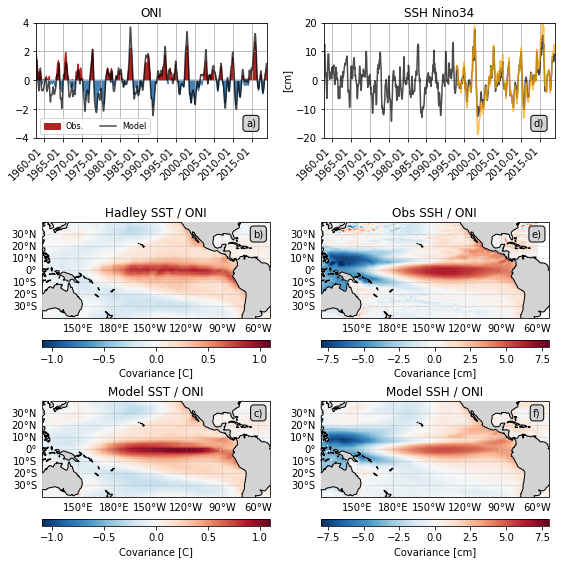
\includegraphics[scale=0.6]{figs/fig1.png}
	\caption{Observed and simulated ONI indexes (a). Covariance between the ONI index and the Hadley (b) and simulated SST anomalies (c). Observed and simulated sea-level anomalies averaged over the Nino34 region (d). Covariances between the ONI index and the observed (e) and simulated (f) sea-level anomalies.}
	\label{fig:nemo-had-sst}
\end{figure}

Modelled ENSO SST  pattern closely resembles the observed one. This pattern is characterized by warm SST anomalies (1°C) centred in the central and eastern equatorial Pacific  flanked by the traditional horseshoe cooling pattern in the western Pacific extending towards the subtropical north and south Pacific. This SST seesaw in the equatorial region is further accompanied by a shoaling of the thermocline in the west and a deepening in the east (not shown).

In addition to SST, satellite-derived sea-level anomalies have been compared with the simulated ones. First, the simulated sea-level anomalies averaged over the Nino34 region compare well with the observed ones (Fig \ref{fig:nemo-had-sst}d), with a correlation coefficient of 0.94. In addition, the spatial patterns associated with ENSO variability are very similar for both the observations and the model (Fig \ref{fig:nemo-had-sst}e, Fig \ref{fig:nemo-had-sst}f). Sea-level anomalies are negative in the western Pacific and positive in the central and eastern Pacific. These anomalies are consistent with thermocline vertical displacements, which shoal in the west and deepends in the east (\warn{REF}).

Covariance maps between the surface chlorophyll and the monthly ONI index are shown in Fig \ref{fig:nemo-sat-chl}. The observations (upper panel) and the model (lower panel) show very similar covariance patterns: El Niño induces a decrease in chlorophyll concentration along the equator east of 150°E, consistent with a weaker equatorial upwelling induced by the equatorial trade winds reduction. However, the model overestimates the chlorophyll response to ENSO variability compared with observational based estimates. Note that the covariance for the simulated chlorophyll has also been computed over the entire simulated period (1958-2018), with no significant changes in the resulting pattern (not shown).

\begin{figure}
	\centering
	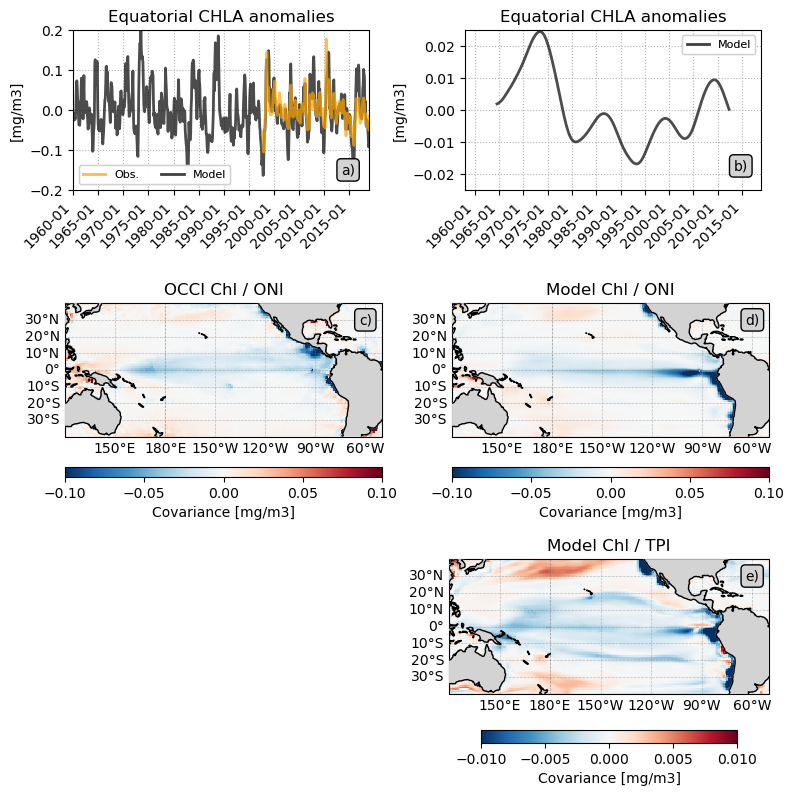
\includegraphics[scale=0.4]{figs/fig2.png}
	\caption{Simulated (black) and observed (yellow) equatorial chlorophyll anomalies (a). Filtered anomalies are shown for the model in panel (b). Covariance between the observed and simulated chlorophyll anomalies with the ONI (c, d) and filtered TPI (e) index.}
	\label{fig:nemo-sat-chl}
\end{figure}

% !TeX root = ../article-enso.tex

\subsection{Marine ecosystem model}
\label{sec:apecosm}

We use the Apex Predators Ecosystem Model (APECOSM, \citealp{mauryModelingEnvironmentalEffects2007, mauryOverviewAPECOSMSpatialized2010}) to simulate the energy transfer through marine ecosystems. 
APECOSM is a eulerian ecosystem model that represents the three-dimensional dynamics of size-structured pelagic populations and communities mechanistically. It integrates individual, population and community levels and includes the effects of life-history diversity with a trait-based approach \citep{mauryIndividualsPopulationsCommunities2013}. In APECOSM, energy uptake and utilization for individual growth, development, reproduction, somatic and maturity maintenance are modeled according to the Dynamic Energy Budget (DEB) theory \citep{koojmanDynamicEnergyBudget2010}. The DEB theory is a comprehensive mechanistic theory of metabolism. It has been extensively tested empirically. In APECOSM, it allows the dynamics of the main components of metabolism and life history and their size, temperature and food dependence to be represented together. In addition to metabolism, APECOSMP considers important ecological processes such as opportunistic size-structured trophic interactions and competition for food, predatory, disease, ageing and starvation mortality, key physiological aspects such as vision and respiration, as well as essential processes such as three-dimensional passive transport by marine currents and active habitat-based movements \citep{faugerasAdvectiondiffusionreactionSizestructuredFish2005}, schooling and swarming (see \citealp{mauryModelingEnvironmentalEffects2007, mauryIndividualsPopulationsCommunities2013, mauryCanSchoolingRegulate2017} for a detailed description of the model). 

As discussed in \cite{mauryIndividualsPopulationsCommunities2013}, size-based predation implies that predation rates are controlled by the ratio of sizes
between prey and predators (all organisms can be potentially predators and
preys at the same time, depending on their relative size, cf. equation D1 of \cite{mauryIndividualsPopulationsCommunities2013} for the detailed equation of the selectivity curve). Opportunistic predation implies that preys
of a given weight are eaten in proportion to their selected
available biomass relatively to the biomass of all possible preys
available.

All the metabolic rates are temperature-dependent and corrected by an Arrhenius factor \citep{mauryModelingEnvironmentalEffects2007, mauryIndividualsPopulationsCommunities2013}. While it can be prescribed in the model configuration, no preferred temperature range has been used in this study. Therefore, while temperature influences metabolism and swimming speed, its horizontal gradient does not influence the direction and magnitude of horizontal active swimming.

In APECOSM, the dynamics of communities is determined by integrating the core state equation below:

\begin{equation}
\partial_t \varepsilon = \underbrace{- \partial_w(\gamma \varepsilon) + \frac{\gamma}{w}\varepsilon}_{Growth} 
\underbrace{- M \varepsilon \vphantom{\frac{\gamma}{w}\varepsilon}}_{Mortalities}
\underbrace{-\overrightarrow{\nabla}.(\overrightarrow{V} \varepsilon) \vphantom{\frac{\gamma}{w}\varepsilon}}_{3D Adv} 
\underbrace{+ \overrightarrow{\nabla} . (D \overrightarrow{\nabla} \varepsilon) \vphantom{\frac{\gamma}{w}\varepsilon}}_{3D Diff.}
\label{eq:apecosm_trend}
\end{equation}

where $\varepsilon$  is the organisms' biomass density in the community, $w$ their individual weight, $\gamma$ is the growth rate, $M$ represents the different mortality rates (computed using equation 12 of \citealt{mauryIndividualsPopulationsCommunities2013}), $V$ and $D$ the sum of 3D passive and active velocities and diffusivity coefficients (computed following \citealt{faugerasAdvectiondiffusionreactionSizestructuredFish2005}). The growth contribution is made of an advection (i.e. the biomass transfer along the size-spectrum, left-hand side) and a source term (i.e. biomass creation, right-hand side). Reproduction is considered through a Dirichlet boundary condition that injects the reproductive outputs from all mature organisms in $w_0$.

In APECOSM, the energy ingested by organisms fuels individual metabolism according to the DEB theory. Ingestion is proportional to a functional Holing type II response function that depends on the size-dependent visibility of prey, their aggregation in schools and temperature. This functional response can be written in a simplified way as follows:

\begin{equation}
f_{c, w} = \dfrac
{P_{c, w}}
{
\dfrac
{C_{c, w} A(T)}
{h_c^{light} s_{c, w}(T)} + P_{c, w}
}
\label{eq:repfonct}
\end{equation}

with $P_{c,w}$ the prey biomass that is available to predator of community $c$ (see \citealt{mauryIndividualsPopulationsCommunities2013} for details) and size $w$, $C_{c,w}$ the half-saturation constant, $A(T)$ the
Arrhenius response of metabolism to temperature $T$, $h_c^{light}$
the response of vision to
ambient light and $s_{c,w}$ the predator speed.

In the APECOSM model, oxygen concentration only modifies the horizontal and vertical habitat of the different communities and size-classes and do not modify, in its current state, the  biological parameters or the physiological rates. Considering the region of interest of the given study, this limitation has barely no consequence. Which would not be the case if analysing outputs within an Oxygen Minimum Zone (OMZ). 

% \begin{displaymath}
% p_{c, u} = \sum_{k=1}^{N_{com}} \left[\int_{v=w_{egg}}^{w_{max}} P^{sch}_{k, v}\ s_{u, v}\ \xi_{k, v}\ dv\right] + \sum_{p=1}^{N_{ltl}} \left[ P^{sch}_{p}\ s_{u, p}\ \xi_{p}\right]
% \end{displaymath}

% \begin{displaymath}
% C_{c, w} = \frac{C_{REF}}{T_{ahr}\times h_c^{light}\times h_c^{tlim}\times W_{w}^{\chi}}
% \end{displaymath}

The APECOSM simulation used in this study is forced by three-dimensional temperature, horizontal current velocities, dissolved oxygen concentration, diatoms, mesozooplankton, microzooplankton and big particulate organic matter carbon concentrations \citep{aumontPISCESv2OceanBiogeochemical2015}, photosynthetically active radiation (PAR) and dynamic layer thickness outputs from the NEMO-PISCES simulation (section \ref{sec:nemo}). Nutrients concentrations simulated by NEMO/PISCES are not used as a forcing to Apecosm.

The APECOSM simulation runs with a daily time step for the biological processes, which is decomposed into a day/night cycle, the duration of which  depends on latitude and day of the year \citep{forsytheModelComparisonDaylength1995}. A sub time-stepping ($dt =0.8h$) is used for horizontal advection and diffusion to ensure numerical stability.

The depth dimension is explicit, i.e. each biological variable (mortality, functional response) is computed in 3 dimensions (depth, latitude, longitude). The vertical distribution is thus determined from habitat functions that depend on the choice of the communities. In this study, three interactive communities are simulated:
\begin{itemize}
\item{The epipelagic community, which includes the organisms that are feeding during the day near the surface such as yellowfin or skipjack tunas for example. Its vertical distribution is influenced by light and visible food during daytime as well as temperature and oxygen during both day and night, while its functional response is influenced by light and temperature.}
\item{The migratory mesopelagic community, which feeds in the surface layer at night and migrates to deeper waters during the day. Its vertical distribution is influenced by light and visible food during the night.}
\item{The resident mesopelagic community, which remains at depth during both night and day. Its vertical distribution is influenced by light and visible food during the day.}
\end{itemize}

To ensure that the size-spectrum is fully unfolded and a pseudo-steady state is achieved, the model was integrated successively over three 1958-2018 cycles. It was first initialized with an arbitrary small biomass value in each size-class and community and integrated from 1958 to 2018 (61 years). Then, the end of this first integration phase was used to run another cycle, which in turn was used to initialize the simulation analyzed in this study.

For each community, equation \ref{eq:apecosm_trend} is integrated over 100 logarithmically distributed size classes, ranging from $0.123cm$ to $196cm$. Since saving the outputs in 3D for the 3 communities and 100 size-classes is very costly, mortality rate, growth rate and functional response for each community and size are vertically averaged as follows:

\begin{equation}
F(y,x,c,w) = \frac{\sum_{z=0}^{H} F(z, y, x, c, w) B(z, y, x, c, w)}{\sum_{z=0}^{H}B(z, y, x, c, w	)}
\end{equation}

with $x$ the longitude, $y$ the latitude, $z$ the depth, $c$ the community, $w$ the size-class, $F$ the variable to consider (functional response, mortality rate, growth rate) and $B$ the 3D biomass (in $J.m^{-3}$).

In the remainder of the paper, the focus is solely put on the response of the epipelagic community; its near-surface location makes it more sensitive to ENSO variability \citep{lemezoNaturalVariabilityMarine2016}, it corresponds to organisms such as skipjack and yellowfin that are targeted by the industrial purse seine fleet, it accounts for the majority of tuna catches in the region, and have been reported to respond markedly to ENSO \citep{lehodeyNinoSouthernOscillation1997}.


%\section{Data and method}
%
%In the present section, the different observation-based datasets used in this study to validate the numerical models are presented. 
%
%%and statistical tools used in this study are presented.
%
%
%
%\subsection{Sea-level anomalies}
%\label{sec:ssh}
%
%Observation-based sea-level anomalies are obtained from the reprocessed Global Ocean Gridded L4 Sea-Surface Heights\footnote{\url{https://doi.org/10.48670/moi-00148}} data, provided by the Copernicus Climate Service as monthly values on a regular $0.25 \times 0.25$ grid from 1993-01 to 2020-12. This product was built by the DUACS multimission altimeter data processing system, which processes data from all altimeter missions: Jason-3, Sentinel-3A, HY-2A, Saral/AltiKa, Cryosat-2, Jason-2, Jason-1, T/P, ENVISAT, GFO, ERS1/2. Using along-track altimeter data, gridded sea-level anomalies are extracted by using an Optimal Interpolation off all the flying satellites. 
%
%%For our study, a monthly sea-level climatology was computed from 1993 to 2018 and used to extract monthly sea-level anomalies, which have been detrended.
%
%\subsection{Chlorophyll}
%\label{sec:chl}
%
%Chlorophyll observation-based estimates are extracted from the monthly OceanColour-CCI V5 CHL-a dataset\footnote{\url{http://dx.doi.org/10.5285/1dbe7a109c0244aaad713e078fd3059a}} \citep{sathyendranathOceanColourTimeSeries2019} over the 1997-09/2018-12 period. For our purpose, the high resolution dataset (4 km) has been regridded on a regular $1\times 1$ grid by computing weighted chlorophyll averages over $24\times24$ boxes, with the weights being provided by the cosine of latitude. When more than $1/3$ of the data used in the averaging is missing, the regridded cell is masked. 
%
%%The monthly climatology has then been computed over the 1998-2008 period and used to extract monthly anomalies, which have then been detrended.
%
%\subsection{Fish biomass estimates}
%\label{sec:fish}
%
%Fish biomass estimates are extracted from the IRD Level 2 global monthly catch of tuna, tuna-like and shark species dataset\footnote{\url{https://doi.org/10.5281/zenodo.1164128}} \citep{taconetGlobalMonthlyCatch2018}. First, the purse-seine captures of skipjack and yellowfin tunas have been extracted from the raw input file. Then, non-monthly observations (i.e. when the difference between the end and start dates exceed 31 days) have been discarded, as well as those which are unlocalized. Finally, the remaining observations have been regridded into on a regular $1 \times 1$ grid using the overlapping area between the observation polygon and the destination cell. The final product is a $3D$ array of dimensions (time and space) that extends from 1959 to 2016. However, due to the early poor data coverage, this dataset was used from 1985 onward.
%
%%\subsection{Covariance analysis}
%%\label{sec:cov}
%%
%%In order to assess the spatial signature of ENSO variability on physical, biogeochemical and biological variables, covariance analysis is used. For each grid cell, the monthly climatology of the analysed fields is removed, and the resulting monthly anomalies are detrended. Finally, the covariance between the detrended anomalies and the ONI index is computed. The resulting map can be interpreted as the monthly anomalies associated with an ONI value of 1.
%%%Correlations are computed in the same way. 
%%%Their significance has been inferred using a Student t-test, in which the effective number of degrees of freedom has been corrected based on the 1-lag autocorrelation of the 2 two time-series \citep{brethertonEffectiveNumberSpatial1999}.